

\documentclass[a4paper,11pt]{article}
\usepackage[german,italian]{babel}
\usepackage{fancyhdr}


\textwidth16cm \textheight24cm \topmargin0mm \headheight0mm
\headsep5mm \oddsidemargin0mm \evensidemargin0mm
\parindent0mm




\usepackage{amsmath}
\usepackage{parskip}
\usepackage{dsfont}
\usepackage{fullpage}
\usepackage{amssymb}
\usepackage{tikz,pgfplots}
\usepackage{cancel}
\usepackage{lmodern}

\usepackage[T1]{fontenc}

\usepackage{theorem}
\usepackage{psfrag}
\usepackage{color}
\usepackage{graphicx}
\usepackage{hyperref}

\usepackage{background}
\usepackage{keystroke}
\usepackage{etoolbox}


\makeatletter
\patchcmd{\tableofcontents}{\@starttoc{toc}}{\hypertarget{totoc}{}\@starttoc{toc}}{}{}
\makeatother

\SetBgScale{1}
\SetBgAngle{0}
\SetBgColor{black}
\SetBgPosition{current page.south}
\SetBgVshift{20pt}
\SetBgContents{\tikz[remember picture,overlay]
    \node[inner sep=0pt] {\hyperlink{totoc}{\Return}};}





\hypersetup{
    colorlinks=true,
    linkcolor=black,
    urlcolor=blue,
    pdftitle={Fourier Analysis Documentation},
    pdfpagemode=FullScreen,
}




\begin{document}




\title{Matematica}

\author{Massimiliano Ferrulli}
\date{04.03.2022}



\maketitle

\section*{Analisi 1}
Teoremi e Definizioni di analisi 1

\pagebreak




\tableofcontents





\pagebreak



\section{Funzioni Reali}

\subsection{Funzione reale di variabile reale}
Definizione:
\\
Dati due sottoinsiemi A e B (non vuoti) di \( \mathbb{R}  \),  una funzione f da A a B associa a ogni numero reale di A uno e uno solo di B

\subsection{Dominio}
Definizione: 
\\
Il dominio naturale di una funzione f è l'insieme più ampio dei valori reale che si possono assegnare alla variabile indipendente x, nel caso y = f(x), affinché esista il corrispondente valore reale \( y \in B \subset \mathbb{R} \) \,

\subsection{Insieme delle immagini}
È l'insieme di valori assunti da una funzione f sul proprio dominio ed è contenuta nel codominio della funzione, con il quale al più può coincidere.

\subsection{Funzione iniettiva}

\begin{center}
\[  
   x_1 \neq x_2 \rightarrow f(x_1) \neq f(x_2)
\]
\end{center}

Una funtione da A a B è iniettiva se ogni elemento di B è immagine di al più un elemento di B
 
\subsection{Funzione Suriettiva}

\begin{center}
    \[
    \forall y \in Cod_f \exists x \in D_f : y=f(x)
    \]
\end{center}
se non specificato il codominio è \( \mathbb{R }\)

\subsection{Funzione periodica}

y=f(x) è una funzione periodica di periodo T, con T > 0

\begin{center}
    \[
    K \in \mathbb{Z} : f(x) = f(x + KT)
    \]
\end{center}

\subsection{Funzioni pari}


\begin{center}
    f(x)=f(-x)
\end{center}

\subsection{Funzione dispari}

\begin{center}
    f(-x) = -f(x)
\end{center}

\subsection{Funzione inversa}
una funzione ammette la funzione inversa \( f^{-1} \) se e solo se è biunivoca 
\begin{center}
    \[
    a = f^{-1} \, b = f(a)
    \]
\end{center}

\subsection{Funzione composta}
Date le funzioni f e g, la funzione composta \( g \circ f \) associa ad ogni x del dominio di f che ha immagine f(x) nel dominio di g il valore y = g(f(x)). 
\\
"Le immagini di fsono il dominio di g"




\section{Limiti}

\subsection{Definizione di funzione continua in un punto}
una funzione definita in un intervallo [a;b] è continua in \(x_0 \in [a;b]\) se e solo se: 
\begin{center}
    \(
    \lim_{x\to x_{0}^+}f(x) =\lim_{x\to x_{0}^-}f(x) = f(x)
    \)
\end{center}

\subsection{punti di discontinuità}
un punto \(x_o\) di f(x) è chiamato punto di discontinuità se f(x) non è continua in \(x_o\).                                  
esistono tre tipi di punti di discontinuità:
un punto \( x_0 \in D_f \) è definito come punto di discontinuità di prima specie se il limite destro e quello sinistro di \( x_0 \) \, ( \( \lim_{x\to x_{0}^+}f(x) \, e \, \lim_{x\to x_{0}^-}f(x) \) ) sono finiti ma con valori diversi.


un punto \(x_0 \in D_f\) è definito come punto di discontinuità di seconda specie se il limite destro e quello sinistro di \(x_0\) \, ( \( \lim_{x\to x_{0}^+}f(x) \, e \, \lim_{x\to x_{0}^-}f(x) \)) sono infiniti oppure non esistono.

un punto \(x_0 \in D_f\) è definito come punto di discontinuità di terza specie se il limite destro e quello sinistro di \(x_0\) \, ( \( \lim_{x\to x_{0}^+}f(x) \, e \, \lim_{x\to x_{0}^-}f(x) \)) coincidono ma sono diversi da \(f(x_0)\)

\subsection{Limite finito per \( x \to x_o \)}

La funzione f(x) ha per limite il numero reale l, per \( x \to x_o \), quando si può determinare un intorno puntato I  di \( x_o \) tale che 


\begin{center}
    \[ 
    \vert f(x) - l\vert < \varepsilon
    \]
\end{center}




\begin{center}
    \[
    \lim_{x \to x_0} f(x) = l \, 
    \text{se} \, 
    \forall \varepsilon > 0 \, \exists I_{\delta} (x_0) : \, 
    \vert f(x) - l \vert < \varepsilon \, ,
    \forall x \in I_{\delta} (x_0) \, 
    x \neq x_0
    \]
\end{center}

\subsection{Limite non finito per \( x \to x_o \)}


\begin{center}
    \[ \bullet
    \lim_{x \to x_0} f(x) = \infty \, 
    \text{se} \, 
    \forall M > 0  \, \exists I_{\delta} (x_0) : \, 
    f(x) > M \, 
    \forall x \in I_{\delta} (x_0) \, 
    x \neq x_0
    \]

\end{center}

nel caso \( - \infty \) :
\begin{center}
    \[ \bullet
    \lim_{x \to x_0} f(x) = - \infty \, 
    \text{se} \, 
    \forall M > 0 \, \exists I_{\delta} (x_0) : \, 
    f(x) < -M \, 
    \forall x \in I_{\delta} (x_0) \, 
    x \neq x_0
    \]

\end{center}

\subsection{Limite finito per \( x \to \infty \) }

\begin{center}
    \[ \bullet
    \lim_{x \to \infty} f(x) = l \, 
    \text{se} \, 
    \forall \varepsilon > 0 \, \exists c > 0 : \, 
    \vert f(x) - l \vert < \varepsilon \, ,
    \forall x > c
    \]

\end{center}

nel caso \( - \infty \) :

\begin{center}
    \[ \bullet
    \lim_{x \to - \infty} f(x) = l \, 
    \text{se} \, 
    \forall \varepsilon > 0 \, \exists c > 0 : \, 
    \vert f(x) - l \vert < \varepsilon \, ,
    \forall x < -c
    \]

\end{center}

\subsection{limite non finito per \( x \to  ^+_-\infty \) }


\begin{center}
    \[ \bullet
    \lim_{x \to \infty} f(x) = \infty \, 
    \text{se} \, 
    \forall M > 0 \, \exists c > 0 : \, 
    f(x) > M  \, ,
    \forall x > c
    \]

\end{center}


\begin{center}
    \[\bullet
    \lim_{x \to - \infty} f(x) = \infty \, 
    \text{se} \, 
    \forall M > 0 \, \exists c > 0 : \, 
    f(x) > M  \, ,
    \forall x <  -c
    \]

\end{center}



\begin{center}
    \[ \bullet
    \lim_{x \to \infty} f(x) = -\infty \, 
    \text{se} \, 
    \forall M > 0 \, \exists c > 0 : \, 
    f(x) < -M  \, ,
    \forall x > c
    \]

\end{center}


\begin{center}
    \[ \bullet
    \lim_{x \to -\infty} f(x) = -\infty \, 
    \text{se} \, 
    \forall M > 0 \, \exists c > 0 : \, 
    f(x) < -M  \, ,
    \forall x < -c
    \]

\end{center}

\subsection{Asintoti}
Un asintoto è una retta alla quale si avvicina indefinitamente una funzione data. 

Asintoto verticale:
\begin{center}
    \[  
        \lim_{x \to x_0 ^- } = \pm \infty \, \text{e/o} \, \lim_{x \to x_0 ^+} = \pm \infty
    \]
\end{center}

Asintoto orizzontale :

\begin{center}
    \[  
        \lim_{x \to \pm \infty} = q
    \]
\end{center}

Asintoto obliquo:

Funzione che converge verso la retta r

\begin{center}
    \[  
        \lim_{x \to  \pm \infty} = \pm \infty
        \hspace{5mm}
        r: y = mx + q 
        \hspace{5mm}
        m = \lim_{x \to  \pm \infty} \frac{f(x)}{x}
        \hspace{5mm}
        q = \lim_{x \to  \pm \infty} f(x) - mx
    \]

\end{center}

\subsection{Teorema dell'unicità del limite}

Enunciato: 

se f(x) ha limite finito l per \(x \to x_0\) allora tale limite è unico

Dimostrazione: 
supponiamo per assurdo che la tesi sia falsa
\begin{center}
    \[
    \lim_{x \to x_o} f(x) = l' \, e \, \lim_{x \to x_o} f(x) = l \hspace{5mm} l' \neq l
    \]
\end{center}

supponiamo \( l<l' \) e scegliamo \(\varepsilon\) tale che 

\begin{center}
    \[
    \varepsilon < \frac{l' - l}{2}
    \]
\end{center}

applichiamo la definizione di limite in entrambi i casi, allora avremo due intorni di \(  x_0 \) : 
\begin{center}
    \[
    \vert f(x) - l \vert < \varepsilon \, \forall x \in I \hspace{5mm}   \vert f(x) - l' \vert < \varepsilon \, \forall x \in I'
    \] 
\end{center}

inoltre \(  I \cap I' \) è un intorno di \(  x_0 \)

in \(  I \cap I' \) devono valere le due disequazioni:

$\begin{cases}
    \vert f(x) - l \vert < \epsilon \\
    \vert f(x) - l' \vert < \epsilon
    \end{cases}$
    $\Longleftrightarrow$
    $\begin{cases}
    l - \epsilon < f(x) < l + \epsilon \\
    l' - \epsilon < f(x) < l' + \epsilon
\end{cases}$

dal confronto delle disuguaglianze ricordando che l < l' risulta che:

\begin{align*}
    l' - \varepsilon < f(x) < l + \varepsilon \to l' - \varepsilon <  l + \varepsilon \\
    \text{ricaviamo}\\
    -2\varepsilon < l - l' \to 2\varepsilon > l' - l
\end{align*}
ciò va contro la nostra ipotesi e dunque la negazione della tesi è falsa e se \(  \lim_{x \to x_0} f(x) = l \) , il limite è unico.

\subsection{Teorema della permanenza del segno}
Se il limite di una funzione per $x \to x_0 = l $ con $l \neq 0$, allora esiste un intorno $\.I _{\delta} (x_0)$ in cui $f(x)$ e $l$ sono entrambi positivi o entrambi negativi.  

\vspace{1mm}

\begin{minipage}{8cm}
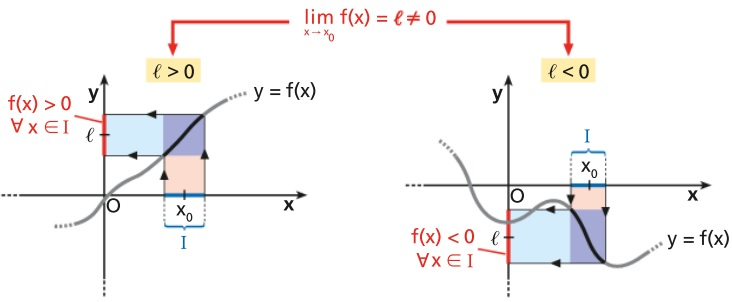
\includegraphics[scale=0.5]{teoremasegno.jpg}
\end{minipage}
\begin{minipage}{8cm}
Il teorema afferma che in un intorno di $x_0$ la funzione $f(x)$ ha lo stesso segno di $l$. Il teorema non è però valido nel caso in cui il limite $l$ sia uguale a 0.
\end{minipage}

\vspace{2mm}

\underline{Dimostrazione:}

\vspace{1mm}

Dalla definizione di $\lim_{x \to x_0} f(x) =l$, scelto qualsiasi $\epsilon$ positivo, deve essere:

$\vert f(x) -l \vert < \epsilon$ \hspace{1mm} $\mapsto$ \hspace{1mm} $l - \epsilon <f(x) < l + \epsilon$.
\hspace{2mm}
Ponendo $\epsilon = \vert l \vert $, si ha: \hspace{1mm}
$l - \vert l \vert < f(x) < l + \vert l \vert $.

Se $l >0$, allora $0<f(x)<2l$ \hspace{1mm} $\mapsto$ \hspace{1mm} $f(x)>0$.

Se $l<0$, allora $2l < f(x) <0$ \hspace{1mm} $\mapsto $ \hspace{1mm} $f(x)<0$.
\hspace{1cm}


\vspace{2mm}

Riprendendo il caso precedenete in cui il teorema non è valido, ovvero quando il limite $l$ è uguale a 0. 
Per esempio, considerando il limite $lim_{x \to 1 } (1-x)=0$ , in un qualunque intorno completo del punto 1, i valori assunti dalla funzione $y=1-x$ sono in parte positivi e in parte negativi. La funzione $f(x)$ è positiva in ogni intorno sinistro di 1 e negativa in ogni intorno destro. Quindi il teorema non è applicabile.

Il teorema della permanenza del segno si può opportunamente invertire; ne segue il teorema:

\vspace{1mm}

Se una funzione $f(x)$ ammette il limite finito $l$ per $x \to x_0$ e in un intorno $I(x_0)$ di $x_0$, escluso al più $x_0$ è:

$\bullet$
Positiva o nulla, allora $l \geqslant  0$;

$\bullet$
Negativa o nulla, allora $l \leqslant 0 $.

\vspace{4mm}

La dimostrazione è ottenibile facendo il processo inverso

\subsection{Teorema del confronto}

Siano $h(x)$, $f(x)$ e $g(x)$ tre funzioni definite in uno stesso intorno $H$ di $x_0$, escluso al più $x_0$. Se in ogni punto di $H$ diverso da $x_0$ risulta $h(x) \leqslant f(x) \leqslant g(x)$ e il limite delle due funzioni $h(x)$ e $g(x)$, per $x$ che tende a $x_0$, è uno stesso numero $l$, allora anche il limite di $f(x)$ per $x \to x_0$ è uguale a $l$.

\vspace{2mm}

Dimostrazione

\vspace{1mm}

Fissiamo $\epsilon > 0$ a piacere, risulta vero che:

\vspace{1mm}

$\vert h(x) - l \vert < \epsilon$, per ogni $x \in I_1 \cap H$ , perché $\lim_{x \to x_0} h(x)=l$;

\vspace{1mm}

$\vert g(x) - l \vert < \epsilon$, per ogni $x \in I_2 \cap H$, perché $\lim_{x \to x_0} g(x)=l$.

Le disuguaglianze valgono entrambe per ogni $x $ appartenente all'intorno $I= I_1 \cap I_2$, escluso al più $x_0$. Quindi per ogni $x \in I$, abbiamo che:

$l - \epsilon < h(x) < l + \epsilon$ \hspace{2mm} , \hspace{2mm}
$l - \epsilon < g(x) < l + \epsilon$.
\hspace{3mm}
Poiché per ipotesi $h(x) \leqslant f(x) \leqslant g(x)$, si scrive:

$l - \epsilon < f(x) < l+ \epsilon$ $\forall x \in I$, ossia:
$\vert f(x) - l \vert < \epsilon $, $\forall x \in I$.
\hspace{5mm}

Questa ultima relazione significa esattamente che $\lim_{x \to x_0} f(x)=l$.

\vspace{1mm}

Esempio:

Sono date le seguenti funzioni:
$h(x)=-x^2 + 4x -2$ , $f(x)=2x-1$, $g(x)=x^2$
\hspace{2mm}
\begin{minipage}{3cm}
\begin{small}
$\lim_{x \to 1 } h(x)=1$ 

\hspace{1mm}

$\lim_{x \to 1 } g(x)=1$
\end{small}
\end{minipage}

\vspace{1mm}

\begin{minipage}{4.5cm}
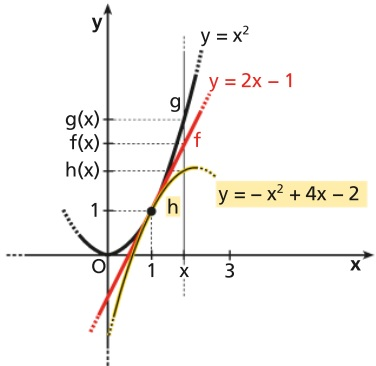
\includegraphics[scale=0.5]{teoremaconfronto.jpg}
\end{minipage}
\begin{minipage}{10cm}
Per $x \to 1$, $h(x)$ e $g(x)$ tendono a 1. Anche $f(x)$, essendo compreso fra $h(x)$ e $g(x)$, deve tendere a 1.

Calcoliamo $\lim_{x \to 1 } f(x)$. Possiamo osservare che per ogni valore $x$ appartenente all'intervallo $]0;3[$, i rispettivi valori delle tre funzioni $h,f$ e $g$ sono, nell'ordine, uno minore uguale dell'altro, ossia: $h(x) \leqslant f(x) \leqslant g(x)$. Il teorema permette allora di affermare che è anche vero che: $\lim_{x \to 1} f(x)=1$.
\end{minipage}

Il teorema vale anche nel caso dei limiti per $x \to \pm \infty$.

\subsection{Teoremi sulle operazioni con le funzioni continue}
Se due funzioni $f(x)$ e $g(x)$, definite nello stesso insieme $\mathcal{D}$, sono continue in un prefissato punto $x_0 \in \mathcal{D}$ allora sono pure continue in $x_0$.

\vspace{1mm}

$\bullet$
Somma: $(f+g)(x)=f(x)+g(x)$

\vspace{1mm}

$\bullet$
Differenza: $(f-g)(x)=f(x)-g(x)$

\vspace{1mm}

$\bullet$
Prodotto: $(f \cdot g)(x)=f(x) \cdot g(x)$

\vspace{1mm}

$\bullet$
Quoziente: $(\frac{f}{g})(x) = \frac{f(x)}{g(x)}$
$\Rightarrow$
Purché $g(x_0) \neq 0$

\subsection{Algebra dei limiti finiti, forme simboliche e di indecisione}
\begin{minipage}{15cm}
    $\bullet$
    $\lim_{x \to x_0} (f(x) \pm g(x))=\lim_{x \to x_0} f(x) \pm \lim_{x \to x_0} g(x) = l \pm m $
    
    \vspace{1mm}
    
    $\bullet$
    $\lim_{x \to x_0} (f(x) \cdot g(x))= \lim_{x \to x_0} f(x) \cdot \lim_{x \to x_0 }g(x) = l \cdot m$
    
    \vspace{1mm}
    
    $\bullet$
    $\lim_{x \to x_0}$
    $\begin{pmatrix}
    \frac{f(x)}{g(x)}
    \end{pmatrix}$
    $= \frac{\lim_{x \to x_0} f(x)}{\lim_{x \to x_0} g(x)} = \frac{l}{m}$
    \hspace{1mm}
    $m \neq 0$
    
    \vspace{1mm}
    
    $\bullet$
    $\lim_{x \to x_0} f(g(x))= f(\lim_{x \to x_0 } g(x))=f(z_0) $
    
    $\bullet$
    $\lim_{x \to x_0} f(x)^{g(x)} = l^m  $
    \vspace{1mm}
    $l,m \neq 0$
    
    \vspace{1mm}
    $\bullet$
    $\lim_{x \to x_0} k \cdot f(x) = k \cdot \lim_{x \to x_0} f(x)= k l$
    
    \vspace{1mm}
    $\bullet$
    $\lim_{x \to x_0} (f(x))^n = (\lim_{x \to x_0} f(x))^n =l^n$
    
    \vspace{1mm}
    $\bullet$
    $\lim_{x \to x_0} \sqrt{f(x)} = \sqrt{\lim_{x \to x_0} f(x)} = \sqrt{l}$
    \end{minipage}
    
    \hspace{0.5mm}
    
    \begin{small}
    
    L'algebra non è più applicabile nei seguenti casi:
    $+ \infty - \infty$, $0 \cdot \infty$, $\frac{\infty}{\infty}$, $\frac{0}{0}$, $1^{\infty}$, $0^0$, $\infty ^0$.
    \end{small}

\subsection{Teorema di Weierstrass}

\label{sec:Weierstrass}

se \(f(x)\) è continua in \([a,b]\) allora assume un massimo assoluto e un minimo assoluto 
\\
cioè esistono \(x_m , x_M \in [a,b]:\)
\begin{align*}
    f(x_m) = m \leq f(x) , \quad x\in [a,b]
    \\
    f(x_M) = M \geq f(x) , \quad x\in [a,b]
\end{align*}
 \(f:[a,b] \rightarrow [m,M]\) se f è continua
\\
\begin{align*}
    \forall \eta \in [m,M] , \quad \exists \xi \in [a,b] : f(\xi) = \eta
\end{align*}

\subsection{Teorema dell'esistenza degli zeri (Bolzano)}

se \(f(x)\) è continua in \([a,b]\) e se \(f(a) * f(b) < 0 \)
\\
allora \( \exists c \in ]a,b[ : f(c) = 0\)

\subsection{Teorema dei valori intermedi}

se \(f(x)\) è continua in \([a,b]\) allora assume almeno una volta tutti i valori intermedi tra il massimo e minimo

\subsection{Metodo di Bisezione}











\section{Calcolo Differenziale}

\subsection{Definizione rapporto incrementale}
data una funzione f(x) definita in un intervallo [a;b], e due numeri reali c , \(c+h \in [a;b]\) \\
 ( \(h \neq 0\) ), il rapporto incrementale di f nel punto c è:
\begin{center}
\(
    \frac{\varDelta y}{\varDelta x} = \frac{f(c+h) - f(c)}{h}
\)    
\end{center}

\subsection{Definizione derivata}
data una funzione f(x) = y definita in un intervallo [a;b], la derivata della funzione nel punto \(c \in [a;b]\) che indichiamo con \(f'(c)\) è il limite, se esiste ed è finito, per \(h \to 0\) del rapporto incrementale di f relativo a c:
\begin{center}
    \(
    f'(c) = \lim_{h \to 0} \frac{f(c+h)-f(c)}{h}
    \)
\end{center}
la derivata di una funzione in un punto c è la pendenza della retta tangente al grafico f nel punto c.

\subsection{teorema sulla continuità e derivabilità di una funzione}

\subsubsection{Enunciato}
Se una funzione f è derivabile in un punto x, allora essa è anche continua in esso.
ipotesi: \(  f'(x_0) = \lim_{h \to 0} \frac{f(x_0+h)-f(x_0)}{h}  \)
tesi: \( \lim_{x \to x_0} f(x) = f(x_0) \)

\subsubsection{Dimostrazione}
\begin{align*}
    f(x_0 + h) &= f(x_0 + h) - f(x_0) + f(x_0) 
    \\
    f(x_0 + h) &= \frac{f(x_0 + h) - f(x_0)}{h} * h + f(x_0)
    \\
    \lim_{h \to 0} f(x_0 + h) &= \lim_{h \to 0} \frac{f(x_0 + h) - f(x_0)}{h} * \lim_{h \to 0} h + f(x_0)  
\end{align*}
\begin{align*}
    \lim_{h \to 0} f(x_0 + h) = f(x_0) 
\end{align*}

\subsection{Teorema di Rolle} 
\subsubsection{Enunciato}
se \(f(x)\) è continua in \([a,b]\) \, derivabile in \(]a,b[\) \, \label{sec:3Rolle} \(f(a) = f(b)\)
\\
allora \( \exists c \in ]a,b[ : f' (c) = 0 \)
\subsubsection{dimostrazione}
per il teorema di \hyperref[sec:Weierstrass]{Weierstrass} la funzione assume un M e un m, quindi esistono \( c,d \in [a,b]\)
\begin{align*}
    m = f(c) \leq f(x) \leq f(d) = M 
\end{align*}
primo caso:
\\
m = m
\\
m = f(c) = f(x) = f(d) = M 
\\
f è quindi costante quindi \( f'(x) = 0 \, \forall x \in [a,b]\)
\\ 
secondo caso:
\\
\( m < M \)
\\
f non è costante e quindi \( f(c+h) \geq f(c) \) cioè \( f(c+h) - f(c) \geq 0 \) 
\begin{align*}
    \frac{f(c+h) - f(c)}{h} \geq 0 
    \\
    h > 0
    \\
    \frac{f(c+h) - f(c)}{h} \leq 0 
    \\
    h < 0
\end{align*}

teorema della permanenza del segno, se esiste un intorno di xo in cui \(f(x) \geq 0 \) e se esiste \( \lim{x \to xo} \, f(x) = l \), allora \( l \geq 0 \)
\\
applicazione

\begin{align*}
  \lim{h \to 0^+} \frac{f(c+h)-f(c)}{h} \geq 0  \, \lim{h \to 0^- } \frac{f(c+h)-f(c)}{h} \leq 0
\end{align*}

due limiti rappresentano derivata destra e sinistra e poiche ( f(x) ) è derivabile, devono essere finiti e coincidenti

\begin{align*}
    f'(c) = \lim{h \to 0} \frac{f(c+h)-f(c)}{h} = 0
\end{align*}

rifare anche per x = d

\subsection{Teorema di Lagrange}
\subsubsection{enunciato}
se \(f(x)\) è continua in \([a,b]\) \, derivabile in \(]a,b[\) 
\\
allora \( \exists \, c \in ]a,b[ : f' (c) = \frac{f(b)-f(a)}{b-a}  \)

\subsubsection{dimostrazione}


Consideriamo:
\begin{center}   
     F(x) = f(x) - kx
    \\
    \text{la funzione F è continua e derivabile essendo f e kx somma di funtioni continue in \([a,b]\) e derivabili in \(]a,b[\) }
    \\
    \text{determiniamo k : rispettiamo la \hyperref[sec:3Rolle]{Terza ipotesi teorema di Rolle}}
\end{center}


\begin{align*}
f(a)- ka = f(b)-kb 
\\
k = \frac{f(b)-f(a)}{b-a} 
\\
F(x) = f(x) - \frac{f(b)- f(a)}{b-a}  x
\end{align*}

F(x) rispetta le ipotesi di Rolle, allora:
\begin{align*}
        \exists \, c \in ]a,b[ : F'(c) = 0
    \\
    F'(c) = f'(c) - \frac{f(b)- f(a)}{b-a} = 0
    \\
    \frac{f(b)- f(a)}{b-a} = f'(c)
\end{align*}

\subsection{ 1a Conseguenza del teorema di Lagrange}
\subsubsection{enunciato}
se \(f(x)\) è continua in \([a,b]\) \, derivabile in \(]a,b[\)  \,  \( f'(x) = 0 \forall x \in ]a,b[\)
\\
allora \( f(x) = k \forall x \in [a,b]  \)

\subsubsection{dimostrazione}

Lagrange in \(]a,x[ x \in [a;b] x \neq a \) 
\\
allora \( \exists c \in ]a;b[ \)

\begin{align*}
    f'c = \frac{f(x)- f(a)}{x-a}
    \\
    f'(x) = 0 \forall x \in  ]a;b[ 
    \\
    f'(c) = 0 
    \\
    f(x) - f(a) = 0 \rightarrow f(x) = f(a) \forall x \in [a;b]
\end{align*}

\subsection{ 2a Conseguenza del teorema di Lagrange}
\subsubsection{enunciato}

se \(f(x)\) e \(g(x)\) sono continue in \([a,b]\) \, derivabili in \(]a,b[\)  \,  \( f'(x)=g'(x) \forall x \in ]a;b[ \)
allora:
\begin{align}
      f(x) = g(x) + k 
\end{align}

\subsubsection{dimostrazione}
\begin{center}
z(x) = f(x) - g(x)  
\\
z'(x) = f'(x) - g'(x) 
\\
f'(x) = g'(x) \text{per ipotesi} 
\\
z'(x) = 0  \text{\(  \forall x \in ]a;b[ \)}
\\
\text{per il teorema precedente} 
\\
z(x) = k \text{\(  \forall x \in [a;b] \)} 
\\
f(x) - g(x) = k
\end{center}

\subsection{Criterio di derivabilità}


\subsubsection{enunciato}

se \(f(x)\) è continua in \([a,b]\) \, derivabile in \(]a,b[\)  a eccezione al massimo di un solo punto \( xo \in ]a;b[\)
\\
allora \(  f'_- (x0) = \lim_{x \to x0_-} f'(x)  \) e \(  f'_+ (x0) = \lim_{x \to x0_+} f'(x)  \)
\\
e se \(  \lim_{x \to x0_-} f'(x) = \lim_{x \to x0_+} f'(x) \)
\\
allora f è derivabile in \(x_0\)
\\
\( f'(x_0) = l \)

\subsubsection{dimostrazione}
se  \(x < x_0\)
    \\
allora  applichiamo Lagrange in \([x;x0]\) dato che f è continua e derivabile nei punti interni  
\\
dunque deve \( \exists c \in ]x;x0[  :  \)
\\

\begin{align*}
    f'c = \frac{f(x)- f(xo)}{x-xo}
\end{align*}

calcoliamo i limiti dei due mebri \( x \to x_0^- \) al primo membro, per definire la derivata sinistra:


\begin{align*}
     f'_-(c) = \lim_{x \to x_0^-}  \frac{f(x)- f(xo)}{x-xo}
\end{align*}
se \( x \to x_0^- \) allora anche \( c \to x_0^- \) quindi per ipotesi si ha:

\begin{align*}
\lim_{c \to x_0^-} f'(c) = l
\end{align*}

quindi 
\begin{align*}
     f'_-(x_0) = l
    \end{align*}

se si risolve in modo analogo considerando \(x < x_0\) ottenendo  \(f'_+(x_0) = l\) 
\\
si concldue che:
\[
    f'(x_0) = l
\]



\subsection{Teorema di Cauchy}
\label{sec:Cauchy}


\subsubsection{Enunciato}
se f(x) e g(x) sono due funzioni continue in [a;b] e derivabili in ]a;b[, \( g'(x) \neq 0 \, \forall x \in [a;b] \) allora:
\[
   \exists c \in [a;b] \, : \, \frac{f(b) - f(a)}{g(b) - g(a)} = \frac{f'(c)}{g'(c)}
\]

\subsubsection{Dimostrazione}

\( F(x) = f(x) - kg(x) \, , \, k \in \mathbb{R} \) \\
F(x) è una funzione continua in [a;b] e derivabile ]a;b[ in quanto somma di funzioni continue e derivabili in questi intervalli. \\
determiniamo k soddisfando \hyperref[sec:3Rolle]{Terza ipotesi teorema di Rolle} cioè F(a) = F(b)
\begin{align*}
f(a) - kg(b) =& f(b) - kg(b)
\\
k =& \frac{f(b) - f(a)}{g(b) - g(a)}    
\\
F(x) = f(x) -& \frac{f(b) - f(a)}{g(b) - g(a)} g(x) 
\end{align*}

F(x) ora soddisfa la \hyperref[sec:3Rolle]{Terza ipotesi teorema di Rolle} e quindi 

\begin{align*}    
\exists c \in ]a;b[ :& F'(c) = 0
\\
F'(c) = 0 = f'(c) -& \frac{f(b) - f(a)}{g(b) - g(a)} g'(c) 
\\
\frac{f(b) - f(a)}{g(b) - g(a)} =& \frac{f'(c)}{g'(c)}
\end{align*}



\subsection{Teorema di De l'Hôpital}

\subsubsection{Enunciato}

date due funzioni f(x) e g(x) definite nell'intorno I di un punto \( x_0 \), se 

$\bullet$
$  f(x) \, g(x) \, \, \, \text{continue in} \, x_0  $
\\
$\bullet$
$  f(x_0) = g(x_0) = 0  $
\\
$\bullet$
$  f(x) \, g(x) \, \, \, \text{derivabili in} \, I \, \text{eccetto al più in} \, x_0 $
\\
$\bullet$
$g'(x) \neq 0 \, \text{in} \,I \, / \, {x_0}$
\\
$\bullet$
esiste $\lim_{x \to x_0} \frac{f'(x)}{g'(x)}$
\\
allora esiste anche $\lim_{x \to x_0} \frac{f(x)}{g(x)}$
\\
$\text{e risulta  } \lim_{x \to x_0} \frac{f(x)}{g(x)} = \lim_{x \to x_0} \frac{f'(x)}{g'(x)} $

\subsubsection{Dimostrazione}

consideriamo un punto qualsiasi \( x \in I \, , \, x \neq x_0 \) e possiamo applicare il teorema di \hyperref[sec:Cauchy]{Cauchy} alle due funzioni f(x) e g(x) nell'intervallo \(  x_0 ; x \) 
\\
allora \( \exists c \in ]x_0 ; x[ \) : 

\[
\frac{f(x) - f(x_0)}{g(x)-g(x_0)} = \frac{f'(c)}{g'(c)}    
\]
per ipotesi \( \frac{f(x)}{g(x)} = \frac{f'(c)}{g'(c)}\)
se \( x \to x_0 \) anche \( c \to x_0\) quindi passando al limite:

\[
\lim_{x \to x_0} \frac{f(x)}{g(x)} =\lim_{c \to x_0} \frac{f'(c)}{g'(c)}      
\]

ma poiché $ \lim_{c \to x_0} \frac{f'(c)}{g'(c)} =  \lim_{x \to x_0} \frac{f'(x)}{g'(x)}  $

\[
    \lim_{x \to x_0} \frac{f(x)}{g(x)} =    \lim_{x \to x_0} \frac{f'(x)}{g'(x)}
\]







\subsection{Teorema di Fermat}




\subsubsection{Enunciato}

Data una funzione $y=f(x)$, definita in un intervallo $[a;b]$ e derivabile in $]a;b[$, se $f(x)$ ha un massimo o un minimo relativo nel punto $x_0$, interno ad $[a;b]$, la derivata della funzione in quel punto $f'(x_0)=0$. 

\vspace{1mm}
 
\subsubsection{Dimostrazione}

Per ipotesi f(x) è derivabile in $x_0$

$\lim_{x \to x_0^-} f'(x) = \lim_{x \to x_0^+} f'(x)$

prendiamo il caso $x_0$ è un massimo

dato un incremento h 

$f(x_0 + h) - f(x_0) \leq 0$

Quindi si ha che:

\vspace{1mm}

$\bullet$
$\frac{f(x_0 + h)-f(x_0)}{h} \leqslant 0$
\hspace{3mm}
$(h>0)$.

\vspace{1mm}

$\bullet$
$\frac{f(x_0 + h)-f(x_0)}{h} \geqslant 0$
\hspace{3mm}
$(h<0)$.

Per l'inverso del teorema della permanenza del segno, risulta che:

\vspace{1mm}

$\lim_{h \to 0^+} \frac{f(x_0 + h)-f(x_0)}{h} \leqslant 0$ \hspace{3mm} e \hspace{3mm}
$\lim_{h \to 0^-} \frac{f(x_0 + h)-f(x_0)}{h} \geqslant 0$.

\vspace{1mm}

Poiché $f(x)$ è derivabile in $x_0$, entrambi i limiti coincidono con $f'(x_0)$. Quindi si ha che:

$f'(x_0) \leqslant 0$ \hspace{3mm} e \hspace{3mm}
$f'(x_0) \geqslant 0$.
\hspace{3mm}
Si conclude quindi che deve essere $f'(x_0)=0$.

\vspace{2mm}

Il teorema afferma che i punti di massimo e di minimo relativo di una funzione derivabile, interni all'intervallo di definizione, sono punti stazionari. Si deduce allora che la tangente in un punto del grafico di massimo o minimo relativo è parallela all'asse $x$.

\vspace{2mm}

In sintesi, il Teorema di Fermat fornisce una condizione necessaria per l'esistenza di un massimo o di un minimo relativo in un punto interno ad $[a;b]$, ma tale condizione non è però sufficiente. Infatti, può accadere che in un punto la retta tangente al grafico della funzione sia parallela all'asse $x$, ma che in quel punto non ci sia né un massimo né un minimo. Ci sarà un flesso. Quindi si può concludere che, data una funzione $y=f(x)$ definita in un intervallo $[a;b]$, i possibili punti di massimo e minimo vanno ricercati tra: I punti in cui $f'(x)=0$, gli estremi dell'intervallo e i punti di non derivabilità.


\end{document}
